\chapter{Convolutional Neural Networks}

When dealing with \textbf{Multilayer Perceptrons} (\textbf{MLP}s), we mostly used data that didn't have articulate structures. Even in the example of the MNIST digits dataset, we still consider the input image as a stream of flattened vectors. This approach, even though helps for making small examples, would not hold well with actual images, which are more complex in terms of number of channels, possible values of each pixel, and so on...
\nl
So how can we deal with that? How can we use images with neural networks, so that to still keep track of relevant informations that would be otherwise lost? The solution is given by the architectural model of the \textbf{Convolutional Neural Network}, CNNs for short. In this first chapter, we'll see how CNNs are made, and what components they have.

\section{Image Filters}

Many times in the fotography field we hear the term \textbf{filter}, but what \textit{is} a filter to begin with? Why do we use it? What kind of filters can we apply? Let's first give a proper definition:

\begin{definition}{Filter}
    A \textbf{filter} is the \textbf{application} of a \textbf{specific function} to a \textbf{local image patch} of a given dimension
\end{definition}

Consider the following example: we have a patch of an image (suppose that the patch's dimensions are smaller than the image ones) and we apply a function which returns the mean of all the pixels adjacent to a selected pixel:

\begin{center}
    \begin{tabular}{c c c}
        \begin{tabular}{|c|c|c|}
            \hline
            8 & 7 & 4 \\
            \hline
            5 & 9 & 1 \\
            \hline
            2 & 3 & 6 \\
            \hline
        \end{tabular} & 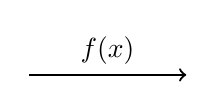
\begin{tikzpicture}
            \draw[black, thick] (0, 0) -- (1, 0) node [anchor = south] {$f(x)$};
            \draw[black, thick, ->] (1, 0) -- (2, 0);
        \end{tikzpicture} & \begin{tabular}{|p{2.2mm}|c|p{2.2mm}|}
            \hline
             & \quad & \\
            \hline
             & 5 & \\
            \hline
             & &  \\
            \hline
        \end{tabular}
    \end{tabular}
\end{center}

Image filtering is a technique that is widely used for various reasons: to \textbf{reduce noise}, to \textbf{fill in missing values} and even to \textbf{extract image features}, such as edges and/or corners. The simplest type of filter that we can have is a filter that replaces each pixel with a linear combination of its neighbours. We call this a \textbf{linear filter}. One of the most known linear filters is the \textbf{2D convolution}.

\begin{definition}{Convolution}
    A \textbf{convolution} is a \textbf{linear filter} which slides a given \textbf{filter kernel} through the image and performs the \textbf{matrix multiplication} between the filter and the overlapped image patch, returning a filtered image.
    \nl
    A filtered image $f$ is expressed as follows:
    \[ f[m, \; n] \eq I \otimes g \eq \sum_{k, \; l} I[m - k, \; n - l] \cdot g[k, \; l] \]

    where $I$ is the image, $g$ is the kernel and $m, \; n, \; k \text{ and } l$ are indexes.
\end{definition}

In the case where in the formula there would've been $+$ instead of $-$ (so within $I[m - k, \; n - l]$), then we would've called that operation a \textbf{correlation}. Let's make a quick example to show how convolutions work:

\begin{example}
    Suppose that we have the following image $I$ and kernel $g$:
    \begin{center}
        \begin{tabular}{c c c}
            \begin{tabular}{|c|c|c|}
                \hline
                8 & 5 & 2 \\
                \hline
                7 & 5 & 3 \\
                \hline
                \textcolor{ForestGreen}{9} & \textcolor{BlueViolet}{4} & \textcolor{BurntOrange}{1} \\
                \hline
            \end{tabular} & \quad & \begin{tabular}{|c|c|p{2.2mm}|}
                \hline
                \textcolor{BurntOrange}{$-1$} & \textcolor{BlueViolet}{0} & \textcolor{ForestGreen}{1} \\
                \hline
                $-1$ & 0 & 1 \\
                \hline
                $-1$ & 0 & 1 \\
                \hline
            \end{tabular} \\
            $I[k, \; l]$ & & $g[k, \; l]$
        \end{tabular}
    \end{center}

    How can we perform the convolution of $I$ with the kernel $g$? Suppose that we want to perform the convolution at the center of the image. When using $k$ and $l$, it's important to note that the coordinates work in the following way:
    \begin{itemize}
        \item the center of the kernel has coordinates $[0, \; 0]$;
        \item if from a coordinate $[k, \; l]$ we move to the right, then we arrive at $[k, \; l - 1]$, and viceversa if we go to the left we arrive to $[k, \; l + 1]$;
        \item if from a coordinate $[k, \; l]$ we move upwards, then we arrive at $[k + 1, \; l]$, and viceversa if we go downwards we arrive to $[k - 1, \; l]$.
    \end{itemize}

    The following schema sums up this coordinate system:
    \begin{center}
        \begin{tabular}{|c|c|c|}
            \hline
            $[1, \; 1]$ & $[1, \; 0]$ & $[0, \; -1]$ \\
            \hline
            $[0, \; 1]$ & $[0, \; 0]$ & $[0, \; -1]$ \\
            \hline
            $[-1, \; 1]$ & $[-1, \; 0]$ & $[-1, \; -1]$ \\
            \hline
        \end{tabular}
    \end{center}

    Now, for $k \eq -1$ and $l \eq -1$, we would have that:
    \[ \textcolor{ForestGreen}{I[m + 1, \; n + 1] \cdot g[-1, \; -1] \eq 1 \cdot -1 \eq -1} \]

    For $k \eq -1$ and $l \eq 0$ we would have instead:
    \[ \textcolor{BlueViolet}{I[m + 1, \; n + 0] \cdot g[-1, \; 0] \eq 4 \cdot 0 \eq 0} \]

    Then, for $k \eq -1$ and $l \eq 1$ we would have:
    \[ \textcolor{BurntOrange}{I[m + 1, \; n - 1] \cdot g[-1, \; 1] \eq 9 \cdot 1 \eq 9} \]

    And so on and so forth for all the multiplications...
\end{example}

From this previous example we had a way to illustrate how the convolution works, but what if we had to code it? If we had to keep track of two different indexes, we would waste some computational memory. Let's try to find a quicker and more efficient method. We can start from the kernel: the multiplication $I \otimes g$ is made between items that are in mirrored positions with respect to some "invisible axes" $l$ and $k$:

\begin{center}
    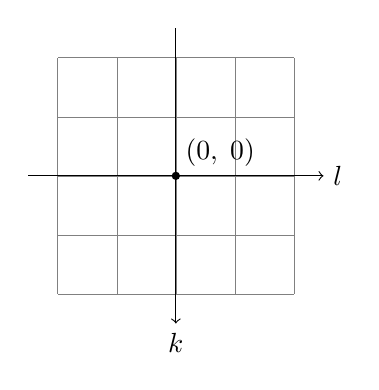
\begin{tikzpicture}[scale = 0.75]
        \draw[step=1cm,gray,very thin] (0, 0) grid (4, -4);
        \draw[black, ->] (-0.5, -2) -- (4.5, -2) node [anchor = west] {$l$};
        \draw[black, ->] (2, 0.5) -- (2, -4.5) node [anchor = north] {$k$};
        \fill[black] (2, -2) circle (2pt) node [anchor = south west] {$(0, \; 0)$};
    \end{tikzpicture}
\end{center}

A simple way to make the computations easier is to flip the kernel along these axes, so that to align it to the image's axes. This way, we would just have to do the element-wise multiplication of the matrices and sum the resulting values.
\nl
A special case of convolution is when we use a 1D filter on a 2D image, but we'll see more about this later on.

\subsection{Linear Filters}

There are different types of filters, depending on the values stored within $g$ and on its shape. For instance, assume that we have a filter whose shape is $1 \times 9$, and that it's equal to the following:
\[ g \eq \begin{bmatrix}
    0 & 0 & 0 & 1 & 0 & 0 & 0
\end{bmatrix} \]

What would it happen if we multiplied $I \otimes g$? For each pixel, the filter would return only the central pixel, so the one in the coordinates $(0, \; 0)$ of the filter when it passes through the image. So, at the end, nothing would change

\begin{center}
    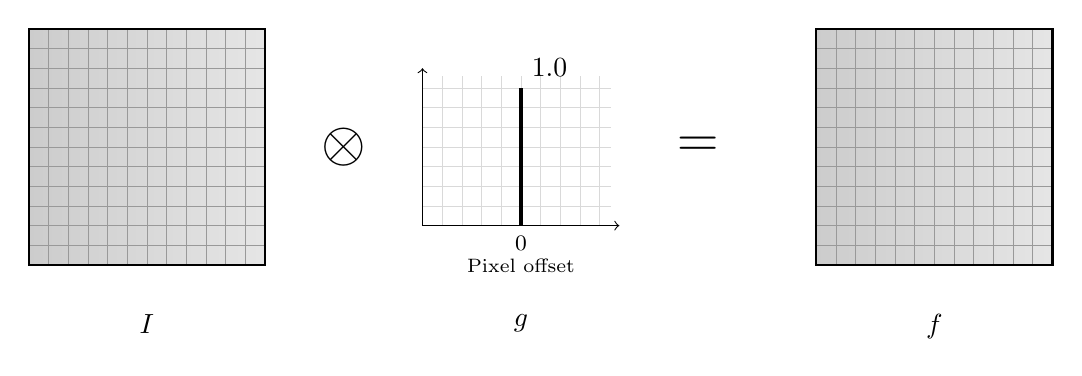
\begin{tikzpicture}
        \fill[left color=gray!40, right color=gray!20] (0, 0) rectangle (3, 3);
        \draw[step=0.25cm, black!40, very thin] (0, 0) grid (3, 3);
        \draw[black, thick] (0, 0) rectangle (3, 3);
        \draw[white] (1.5, -0.5) circle (0.1pt) node [anchor = north] {\textcolor{black}{$I$}};

        \draw[white] (4, 1.5) circle (0.1pt) node [anchor = center] {\textcolor{black}{\huge$\otimes$}};

        \draw[step=0.25cm, gray!30, very thin] (5, 0.5) grid (7.40, 2.40);
        \draw[black, ->] (5, 0.5) -- (7.5, 0.5);
        \draw[black, ->] (5, 0.5) -- (5, 2.5);
        \draw[white] (6.25, 0.49) circle (0.1pt) node [anchor = north] {\textcolor{black}{\footnotesize$0$}};
        \draw[white] (6.25, 0.2) circle (0.1pt) node [anchor = north] {\textcolor{black}{\scriptsize Pixel offset}};
        \draw[white] (6.25, -0.5) circle (0.1pt) node [anchor = north] {\textcolor{black}{$g$}};
        
        \draw[black, very thick] (6.25, 0.5) -- (6.25, 2.25) node [anchor = south west] {$1.0$};

        \draw[white] (8.5, 1.5) circle (0.1pt) node [anchor = center] {\textcolor{black}{\huge$=$}};

        \fill[left color=gray!40, right color=gray!20] (10, 0) rectangle (13, 3);
        \draw[step=0.25cm, black!40, very thin] (10, 0) grid (13, 3);
        \draw[black, thick] (10, 0) rectangle (13, 3);
        \draw[white] (11.5, -0.5) circle (0.1pt) node [anchor = north] {\textcolor{black}{$f$}};
    \end{tikzpicture}
\end{center}

What if we used instead the following filter $g$?
\[ g \eq \begin{bmatrix}
    1 & 0 & 0 & 0 & 0 & 0 & 0 & 0 & 0
\end{bmatrix} \]

Now, for each pixel on which the filter slides, we would take a pixel that is 3 pixels at the right and place it at the local coordinates $(0, \; 0)$. If we repeat that for the entire image, we will then obtain an image shifted by 3 pixels:

\begin{center}
    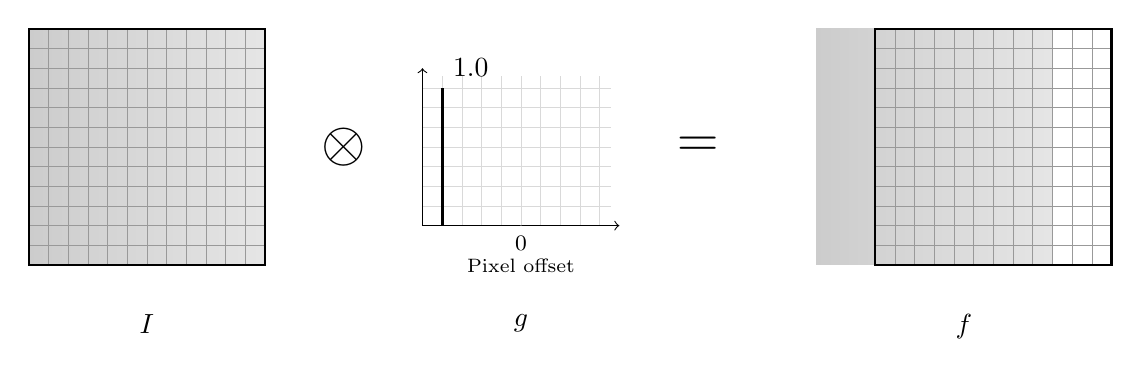
\begin{tikzpicture}
        \fill[left color=gray!40, right color=gray!20] (0, 0) rectangle (3, 3);
        \draw[step=0.25cm, black!40, very thin] (0, 0) grid (3, 3);
        \draw[black, thick] (0, 0) rectangle (3, 3);
        \draw[white] (1.5, -0.5) circle (0.1pt) node [anchor = north] {\textcolor{black}{$I$}};

        \draw[white] (4, 1.5) circle (0.1pt) node [anchor = center] {\textcolor{black}{\huge$\otimes$}};

        \draw[step=0.25cm, gray!30, very thin] (5, 0.5) grid (7.40, 2.40);
        \draw[black, ->] (5, 0.5) -- (7.5, 0.5);
        \draw[black, ->] (5, 0.5) -- (5, 2.5);
        \draw[white] (6.25, 0.49) circle (0.1pt) node [anchor = north] {\textcolor{black}{\footnotesize$0$}};
        \draw[white] (6.25, 0.2) circle (0.1pt) node [anchor = north] {\textcolor{black}{\scriptsize Pixel offset}};
        \draw[white] (6.25, -0.5) circle (0.1pt) node [anchor = north] {\textcolor{black}{$g$}};
        
        \draw[black, very thick] (5.25, 0.5) -- (5.25, 2.25) node [anchor = south west] {$1.0$};

        \draw[white] (8.5, 1.5) circle (0.1pt) node [anchor = center] {\textcolor{black}{\huge$=$}};

        \fill[left color=gray!40, right color=gray!20] (10, 0) rectangle (13, 3);
        \draw[step=0.25cm, black!40, very thin] (10.75, 0) grid (13.75, 3);
        \draw[black, thick] (10.75, 0) rectangle (13.75, 3);
        \draw[white] (11.875, -0.5) circle (0.1pt) node [anchor = north] {\textcolor{black}{$f$}};
    \end{tikzpicture}
\end{center}

A very interesting filter is the following:
\[ g \eq \begin{bmatrix}
    0 & 0 & 0 & 0,33 & 0,33 & 0,33 & 0 & 0 & 0
\end{bmatrix} \]

\noindent This filter combines a pixel with its neighbours, taking a third of each pixel's values and then summing them up together. This kind of filter is called \textbf{blur}.

\begin{center}
    \begin{tikzpicture}
        \draw[white] (1.5, 1.5) circle (0pt) node [anchor = center] {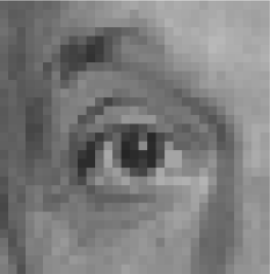
\includegraphics[width = 3cm, height = 3cm]{imgs/001.png}};
        \draw[black, thick] (0, 0) rectangle (3, 3);
        \draw[white] (1.5, -0.5) circle (0.1pt) node [anchor = north] {\textcolor{black}{$I$}};

        \draw[white] (4, 1.5) circle (0.1pt) node [anchor = center] {\textcolor{black}{\huge$\otimes$}};

        \draw[step=0.25cm, gray!30, very thin] (5, 0.5) grid (7.40, 2.40);
        \draw[black, ->] (5, 0.5) -- (7.5, 0.5);
        \draw[black, ->] (5, 0.5) -- (5, 2.5);
        \draw[white] (6.25, 0.49) circle (0.1pt) node [anchor = north] {\textcolor{black}{\footnotesize$0$}};
        \draw[white] (6.25, 0.2) circle (0.1pt) node [anchor = north] {\textcolor{black}{\scriptsize Pixel offset}};
        \draw[white] (6.25, -0.5) circle (0.1pt) node [anchor = north] {\textcolor{black}{$g$}};
        
        \draw[black, very thick] (5.25, 0.5) -- (5.25, 2.25) node [anchor = south west] {$1.0$};

        \draw[white] (8.5, 1.5) circle (0.1pt) node [anchor = center] {\textcolor{black}{\huge$=$}};

        \draw[white] (11.5, 1.5) circle (0pt) node [anchor = center] {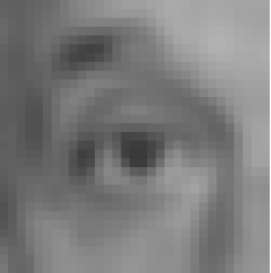
\includegraphics[width = 3cm, height = 3cm]{imgs/002.png}};
        \draw[black, thick] (10, 0) rectangle (13, 3);
        \draw[white] (11.5, -0.5) circle (0.1pt) node [anchor = north] {\textcolor{black}{$f$}};
    \end{tikzpicture}
\end{center}

When dealing with images, it's important to also recognize some details, such as an edge or some variations in the color. But how do we define them?

\begin{definition}{Edge}
    An \textbf{edge} of an image is when there is an \textbf{abrupt change} of the values from one pixel to an adjacent one
\end{definition}

Also, it's possible that we can sometimes deal with \textbf{impulses}, so images where only one pixel stores non-zero values.
\nl
Generally, it's important to recognize edges in the images because it helps on detecting items. But not in all images the edges are clear to recognize, and sometimes we may need to accentuate, to \textbf{sharp} them. This can be done through a \textbf{sharpening filter}, which usually has the following form:

\begin{center}
    \begin{tikzpicture}
        \draw[white] (1.5, 1.5) circle (0pt) node [anchor = center] {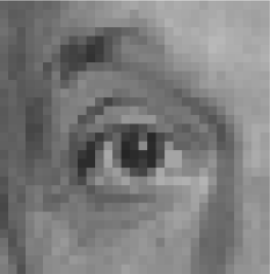
\includegraphics[width = 3cm, height = 3cm]{imgs/001.png}};
        \draw[black, thick] (0, 0) rectangle (3, 3);
        \draw[white] (1.5, -1) circle (0.1pt) node [anchor = north] {\textcolor{black}{$I$}};

        \draw[white] (4, 1.5) circle (0.1pt) node [anchor = center] {\textcolor{black}{\huge$\otimes$}};

        \draw[step=0.25cm, gray!30, very thin] (5, 0.5) grid (7.40, 2.40);
        \draw[black, ->] (5, 0.5) -- (7.5, 0.5);
        \draw[black, ->] (5, 0.5) -- (5, 2.5);
        \draw[white] (6.25, 0) circle (0.1pt) node [anchor = north] {\textcolor{black}{\footnotesize$0$}};
        \draw[white] (6.25, -0.29) circle (0.1pt) node [anchor = north] {\textcolor{black}{\scriptsize Pixel offset}};
        \draw[white] (6.25, -1) circle (0.1pt) node [anchor = north] {\textcolor{black}{$g$}};
        
        \draw[black, very thick] (6.25, 0.5) -- (6.25, 2.75) node [anchor = south west] {$1.\overline{6}$};
        \draw[black, very thick] (6, 0.5) -- (6, 0.2) node [anchor = east] {$0.\overline{3}$};
        \draw[black, very thick] (6.50, 0.5) -- (6.50, 0.2) node [anchor = west] {$0.\overline{3}$};

        \draw[white] (8.5, 1.5) circle (0.1pt) node [anchor = center] {\textcolor{black}{\huge$=$}};

        \draw[white] (11.5, 1.5) circle (0pt) node [anchor = center] {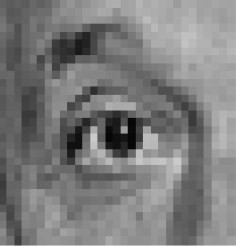
\includegraphics[width = 3cm, height = 3cm]{imgs/003.png}};
        \draw[black, thick] (10, 0) rectangle (13, 3);
        \draw[white] (11.5, -1) circle (0.1pt) node [anchor = north] {\textcolor{black}{$f$}};
    \end{tikzpicture}
\end{center}

We can notice how the differences of colors are accentuated, and how the costant areas are instead left similar to the original image.
\nl
Since these filters are all linear, they also can use the basic properties of the linear systems, which are the following three:
\begin{itemize}
    \item \textbf{Homogeneity}: $T[a \cdot X] \eq a \cdot T[X]$;
    \item \textbf{Additivity}: $T[X_1 + X_2] \eq T[X_1] + T[X_2]$;
    \item \textbf{Superposition}: $T[a \cdot X_1 + b \cdot X_2] \eq a \cdot T[X_1] + b \cdot T[X_2]$.
\end{itemize}

In general, a system is said to be \textbf{linear} if and only if the \textbf{superposition} property \textbf{holds}. All the filters presented until now are linear filters (convolutions too), so they can take advantage of these properties.

\subsection{Average and Gaussian Filters}

There are other interesting types of filters that we can use with convolutions, such as the \textbf{average filter}. The task of this filter is to replace each pixel with an average of its neighbours (so for instance, each neighbour of a pixel will contribute to $\nicefrac{1}{9}$ of the total value). The average can also have different \textbf{weights}, so that to give more importance to some pixels than to others. If all the weights are equal, then such filter is also called \textbf{box filter}.
\nl
Another type of blur filter is the \textbf{Gaussian Average filter}, which weights the neighbours depending on their distance from the central pixel (the nearer, the greater the weight). The smoothing of the kernel is proportional to the Gaussian function:
\[ \underbrace{g}_{\text{kernel}} \; \propto \; \underbrace{\frac{1}{2 \pi \sigma^2} \cdot e^{- \frac{x^2 + y^2}{2 \sigma^2}}}_{\text{Gaussian function}} \]

We can here compare the results of the average and Gaussian filters:
\begin{center}
    \footnotesize
    \begin{tabular}{c c c}
        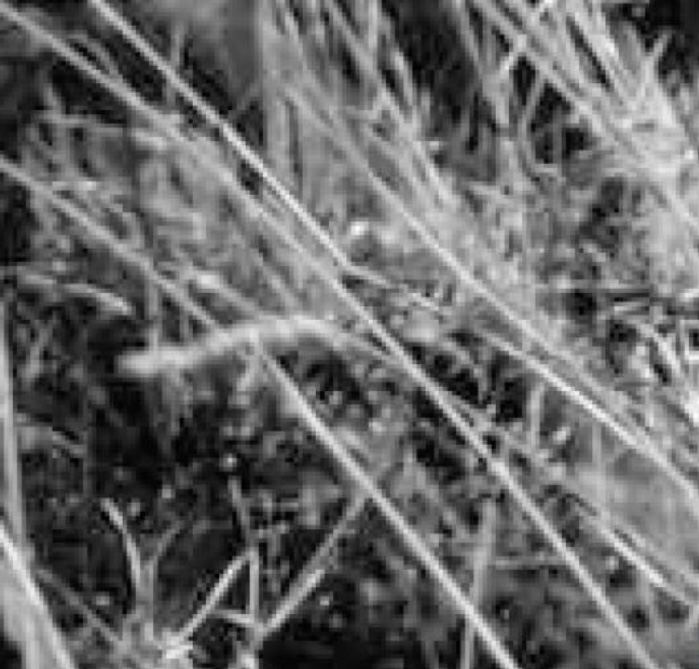
\includegraphics[width = 4cm]{imgs/004.jpg} & 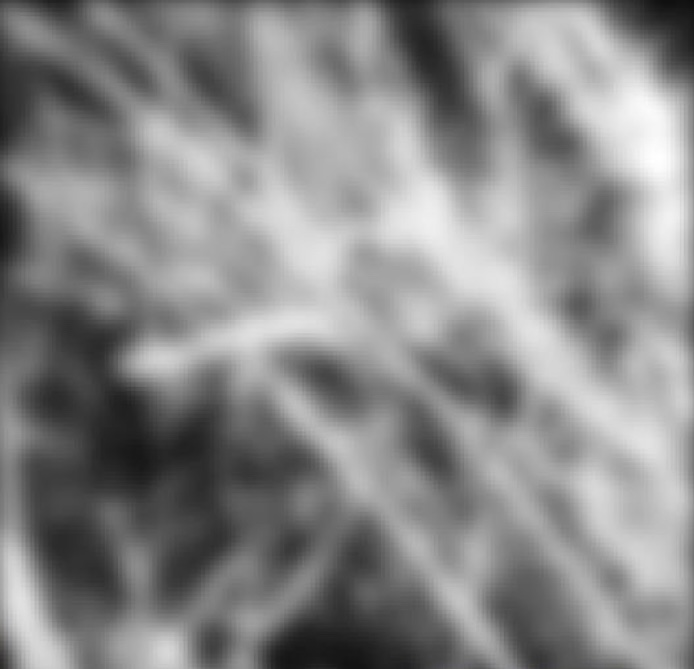
\includegraphics[width = 4cm]{imgs/005.jpg} & 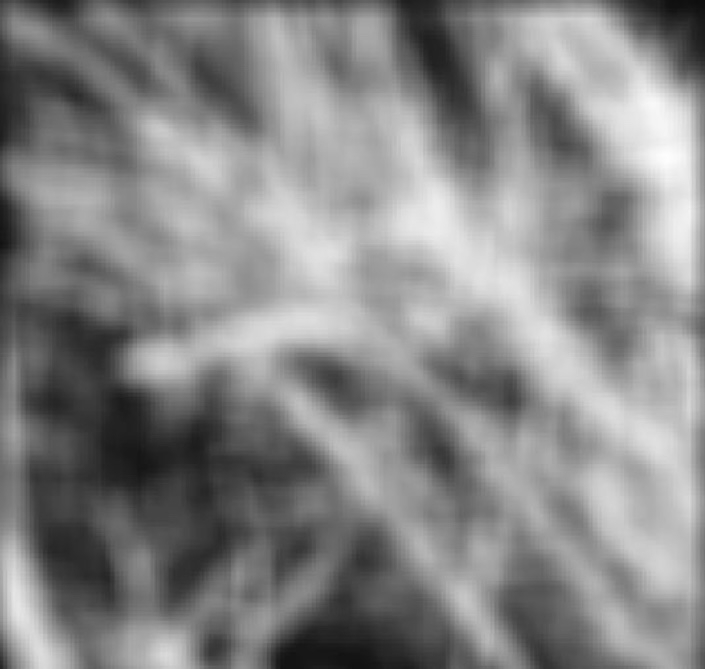
\includegraphics[width = 4cm]{imgs/006.jpg} \\
        \textbf{Starting image $I$} & \textbf{Average Filter} & \textbf{Gaussian Filter}
    \end{tabular}
\end{center}

The utility of the box filter and the Gaussian filters is that they are \textbf{separable}, which means that we can first convolve the rows with a one dimensional filter and then convolve the columns with another one dimensional filter. This is very \textbf{efficient} when it comes to computing the filters, because with the full box filter for instance we would have to do $k^2 \cdot n$ operations, but with the separated box filters we would only have to do $2k \cdot n$ operations. This is possible because the \textbf{convolution is linear}, so we can use the associative and commutative operations.

\[ (f_x \otimes f_y) \otimes I \eq f_x \otimes (f_y \otimes I) \]

\subsection{Edges and Derivatives}

When we have an image with abrupt changes of values, we say that we have an \textbf{edge}. But how can we detect such edges mathematically? Suppose that we have the following image:

\begin{center}
    \begin{tabular}{c c}
        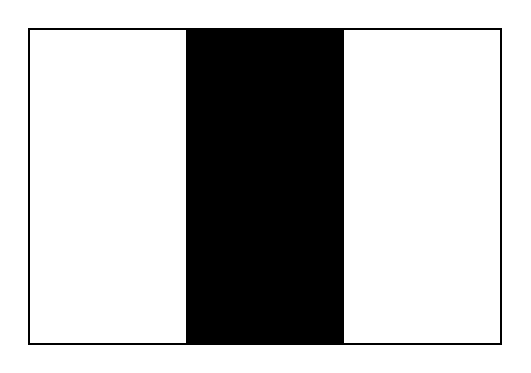
\begin{tikzpicture}
            \draw[black, thick] (0, 0) rectangle (6, 4);
            \fill[black] (2, 0) rectangle (4, 4);
        \end{tikzpicture} &
        \raisebox{54pt}{$\begin{bmatrix}
            255 & ... & 255 & 0 & ... & 0 & 255 & ... & 255 \\
            255 & ... & 255 & 0 & ... & 0 & 255 & ... & 255 \\
            255 & ... & 255 & 0 & ... & 0 & 255 & ... & 255 \\
            255 & ... & 255 & 0 & ... & 0 & 255 & ... & 255 \\
            255 & ... & 255 & 0 & ... & 0 & 255 & ... & 255 \\
            255 & ... & 255 & 0 & ... & 0 & 255 & ... & 255 \\
        \end{bmatrix}$}
    \end{tabular}
\end{center}

We see how we have an abrupt change of values from $255$ to $0$. We can exploit derivatives to see the behaviour of the function. Indeed, if we compute the first derivative, we obtain the following matrix:
\nl
\[\begin{bmatrix}
    0 & ... & 0 & 255 & 0 & ... & 0 & -255 & 0 & ... & 0 \\
    0 & ... & 0 & 255 & 0 & ... & 0 & -255 & 0 & ... & 0 \\
    0 & ... & 0 & 255 & 0 & ... & 0 & -255 & 0 & ... & 0 \\
    0 & ... & 0 & 255 & 0 & ... & 0 & -255 & 0 & ... & 0 \\
    0 & ... & 0 & 255 & 0 & ... & 0 & -255 & 0 & ... & 0 \\
    0 & ... & 0 & 255 & 0 & ... & 0 & -255 & 0 & ... & 0 \\
\end{bmatrix}\]
\nl
As we can see, the values $255$ and $-255$ denote where we have a change of values in the image. This allows us to detect eventual changes in the image. We can also compute the second derivative, which will allow us to gain further intel about which color is changing to which.